\chapter{Interfacce}
\section{Modi}
\begin{redbar}
Nel design dell’interazione uomo-macchina, i \textbf{modi} rappresentano uno dei concetti chiave per la gestione delle risposte del sistema ai comandi dell’utente. Un'interfaccia è definita “modale” quando il significato di un gesto cambia a seconda dello stato attuale del sistema. 
\end{redbar}

I modi determinano come un'interfaccia interpreta un'azione specifica dell'utente, come un clic o un gesto, variando il suo comportamento a seconda delle impostazioni o dei contesti attivi.

Prima di analizzare i modi, è essenziale comprendere alcuni termini chiave:
\begin{itemize}
    \item \textit{Content:} rappresenta l'insieme delle informazioni presenti nel sistema, significative e utili per l'utente.
    \item \textit{GID (Graphical Input Device):} è un dispositivo grafico di input, come il mouse, che permette di comunicare la posizione del cursore o la selezione di un oggetto.
    \item \textit{GID Button:} è il tasto principale del GID, utilizzato per selezionare o attivare elementi.
    \item \textit{Tap:} si riferisce all'azione di premere e rilasciare un tasto, come il tocco su uno schermo o la pressione su un mouse.
    \item \textit{Click, Double-Click, Drag e Swipe:} questi termini indicano azioni di interazione comune. Ad esempio, il click rappresenta una singola pressione, mentre il drag prevede il trascinamento di un oggetto mantenendo premuto il pulsante.
\end{itemize}
Una \textit{gesture} (o gesto) rappresenta una sequenza di azioni completata automaticamente una volta avviata. I modi descrivono il modo in cui un'interfaccia risponde ai gesti. Se un'interfaccia interpreta un gesto sempre nello stesso modo, allora si trova in un unico modo. Tuttavia, se l'interpretazione del gesto cambia a seconda dello stato del sistema, ci troviamo di fronte a un'interfaccia in modalità variabile. Ad esempio, il tasto “Invio” potrebbe servire per andare a capo in un documento o per confermare un comando in una finestra di dialogo. L’interfaccia, quindi, assume significati diversi per lo stesso gesto, a seconda dello stato in cui si trova.

\begin{Example}{Torcia e sveglia}{}
\textit{Prendiamo ad esempio una torcia che si accende e si spegne con un pulsante a pressione.}

Quando è in tasca, non possiamo prevedere con sicurezza cosa accadrà premendo il pulsante, poiché non è visibile lo stato del sistema (accesa o spenta). Questo richiede una verifica separata dello stato della torcia.

\textit{Un altro esempio comune è la sveglia con un pulsante per attivarla o disattivarla.} 

Se la sveglia è attiva e si preme il pulsante, questa si disattiva, e viceversa. Al buio, non vedendo il display, non è possibile conoscere lo stato attuale della sveglia e prevedere l’effetto della pressione del pulsante.
\end{Example}

Il \textit{luogo dell'attenzione} è un concetto che rappresenta l'oggetto fisico o mentale su cui l'utente concentra intenzionalmente la sua attenzione. È importante notare che l'utente può avere un solo luogo dell'attenzione alla volta. Se un cambiamento o un'azione si verifica al di fuori di questo luogo, è possibile che l'utente non se ne accorga, causando potenziali errori.

\begin{Example}{Caps lock}{}
Il tasto Caps Lock crea un modo: quando attivato, tutte le lettere digitate sono maiuscole. È un errore comune iniziare a scrivere e accorgersi solo dopo alcune parole che il blocco maiuscole è attivo. Sebbene un LED verde sul tasto stesso segnali chiaramente lo stato attuale, e alcune applicazioni visualizzino un indicatore nella barra di stato, l’errore persiste. Ciò accade perché l'utente si focalizza sul contenuto digitato, non sullo stato di Caps Lock, situato fuori dal suo luogo dell'attenzione.
\end{Example}

\subsection{Errori di modo}
I modi possono essere utili in alcune situazioni per aumentare la flessibilità, ma possono anche portare a errori. L'esperienza di un utente non elimina la possibilità di errori legati ai modi, poiché l'esperto ha sviluppato abitudini che potrebbero renderlo più vulnerabile a fraintendimenti in caso di cambiamenti nella modalità.

Gli errori di modo, ossia gli errori causati da una valutazione sbagliata dello stato del sistema, possono essere ridotti seguendo alcuni principi:
\begin{enumerate}
    \item Evitare i modi quando possibile.
    \item Segnalare chiaramente i modi presenti.
    \item Distinguere i comandi in base ai modi: in modo che un comando emesso nel modo errato non produca effetti indesiderati.
\end{enumerate}
Un'interfaccia è \textit{modale} se
\begin{enumerate}
    \item lo stato corrente dell'interfaccia non è il luogo dell'attenzione dell'utente e
    \item se rispetto a un gesto può rispondere a quel gesto in diversi modi a seconda dello stato del sistema.
\end{enumerate}
Invece, un'interfaccia è completamente \textit{non-modale} se risponde sempre nello stesso modo a ogni gesto possibile. È possibile misurare il grado di "modularità" di un'interfaccia attraverso la probabilità che un gesto venga interpretato in modo non ambiguo, con 0 che indica un'interfaccia completamente modale e 1 un'interfaccia totalmente non modale.

Alcuni modi sono \textit{modi temporanei} e svaniscono dopo l’uso (ad esempio, l’uso del pennello in Word attivato con un singolo clic), mentre altri sono \textit{quasi-modi}, attivi finché si mantiene premuto un controllo, come il tasto Shift o CTRL.

\subsection{Noun-verb e verb-noun}
Le azioni in un'interfaccia possono essere strutturate in due modi:
\begin{enumerate}
    \item \textit{Noun-Verb:} si seleziona prima l’oggetto e poi si sceglie l’azione da eseguire su di esso.
    \item \textit{Verb-Noun:} si seleziona prima l’azione e poi l’oggetto.
\end{enumerate}
Entrambi i metodi hanno vantaggi e svantaggi, influenzando il flusso naturale dell'attenzione dell'utente e la facilità di completamento dell’azione.

Ad esempio, cambiare il font di un testo rappresenta un’interazione noun-verb (prima si seleziona il testo, poi si applica il font). La selezione di un tool in una palette di strumenti è invece un esempio di verb-noun (prima si sceglie lo strumento, poi si applica all’oggetto).

Nell'approccio verb-noun, l'utente è spinto a focalizzare il luogo dell'attenzione sull'azione da compiere, selezionandola per prima. Una volta selezionata l’azione, l'utente sposta il suo focus sull'oggetto. Tuttavia, questo approccio può portare a errori di modo, specialmente se l'utente si distrae o il luogo dell’attenzione viene spostato in modo imprevisto. Questo tipo di interazione richiede, infatti, un doppio cambio del luogo dell'attenzione: dall'azione inizialmente selezionata all'oggetto su cui essa va applicata.

D'altra parte, l'approccio noun-verb si caratterizza per la selezione iniziale dell'oggetto che è già nel luogo dell'attenzione dell'utente. In questo caso, una volta scelto l'oggetto, il luogo dell'attenzione si sposta solo sull'azione, riducendo il numero di passaggi e spostamenti necessari per completare l’operazione. Questo tipo di sequenza offre vantaggi significativi in termini di semplicità e reversibilità dell'azione: interrompere un'operazione richiede soltanto di deselezionare l’oggetto, senza bisogno di confermare o annullare l'azione.

\begin{Example}{Sistema per richiedere prodotti}{}
\textit{Consideriamo il caso di un sistema progettato per richiedere prodotti in una multinazionale.}

Nel flusso originale, basato sul modello verb-noun, all'utente veniva richiesto di selezionare per prima cosa il dipartimento a cui i prodotti sarebbero stati inviati. Solo in seguito poteva scegliere gli articoli desiderati. Questo processo, seppur strutturato, portava a confusione e a errori. In particolare, il sistema impostava di default il dipartimento associato alla postazione in uso, ma se l’utente si trovava temporaneamente in un altro dipartimento, spesso dimenticava di cambiare l'impostazione, causando così l’invio degli articoli a un luogo sbagliato. Questo errore derivava dal fatto che l’ordine delle azioni non seguiva il flusso naturale dell'attenzione dell’utente, il quale si concentrava prima sugli articoli necessari e solo successivamente sul luogo di destinazione.

Per risolvere questi problemi, è stata introdotta una modifica al flusso, trasformandolo in un processo di tipo noun-verb. La soluzione prevedeva di mettere in cima all'interfaccia la scelta degli articoli, come primo passo dell’ordine. Inoltre, è stata aggiunta una descrizione chiara: "A quale dipartimento vuoi che gli articoli siano inviati?" per guidare meglio l’utente. Il sistema è stato inoltre modificato per identificare automaticamente il dipartimento dell’utente tramite il login, con l’opzione “Il mio dipartimento” come prima voce nella lista.

Questa nuova interfaccia ha portato diversi vantaggi. In primo luogo, la scelta del dipartimento è diventata un’azione finale, che completa logicamente il processo. Questo cambiamento ha contribuito a ridurre gli errori e a migliorare il flusso naturale dell'attenzione dell'utente, il quale non è più costretto a ricordare di cambiare il dipartimento predefinito. Infine, è stata eliminata la necessità di un click finale di conferma, riducendo così il numero di azioni richieste per completare l'ordine.
\end{Example}

\section{Affordances e signifiers}
Il concetto di \textit{affordance}, introdotto dallo psicologo Don Norman:
\begin{center}
\textit{"una relazione tra le proprietà di un oggetto e le capacità dell'agente che determinano esattamente come l'oggetto potrebbe essere utilizzato"}
\end{center}
In altre parole, la forma, la dimensione e l'aspetto dell'oggetto suggeriscono implicitamente quali azioni l’utente può compiere.

\begin{figure}[ht]
    \centering
    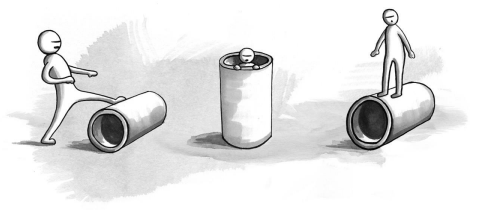
\includegraphics[width=0.5\linewidth]{images/affordance.PNG}
    \caption{Affordance}
    \label{fig:affordance}
\end{figure}

L’affordance dipende sia dall'oggetto sia dall'utente. Se l'utente possiede le capacità percettive per comprendere come usare l'oggetto, allora l'affordance può guidarlo verso l’azione corretta. Tuttavia, in alcuni casi, le affordance non sono ovvie, o possono addirittura essere "nascoste", portando l'utente a fraintendimenti.

La famosa frase di Eleanor Gibson, \textit{"percepiamo per imparare, così come impariamo per percepire"} illustra come l’interazione tra percezione e azione sia fondamentale. Questo principio viene evidenziato dal celebre esperimento del “visual cliff” (baratro visivo), in cui i neonati venivano messi su una piattaforma trasparente sospesa sopra il suolo. L'esperimento dimostrava come la percezione del baratro induceva i bambini a evitare l'area, dimostrando la percezione immediata di un affordance che suggeriva pericolo.

Mentre le affordances sono caratteristiche intrinseche degli oggetti, i signifiers sono indicatori percepibili che comunicano all’utente quale comportamento adottare con un oggetto. Don Norman li definisce come 
\begin{center}
    \textit{"qualsiasi segno, simbolo, suono o altro indicatore percepibile che guida l'utente verso l'azione corretta"}
\end{center}
I signifiers includono elementi come etichette, frecce, simboli o icone che rendono esplicite le azioni desiderate. Ad esempio, un cartello con scritto "spingere" o "tirare" su una porta è un signifier che elimina ogni ambiguità su come aprirla.

Nelle interfacce uomo-macchina, i signifiers svolgono un ruolo fondamentale per guidare l'utente. Poiché l’interazione con i sistemi digitali può essere meno intuitiva rispetto agli oggetti fisici, i signifiers diventano più rilevanti delle affordances. I signifiers visivi e uditivi sono particolarmente utili per rendere chiaro cosa l’utente può fare in ogni momento, riducendo così l’incertezza.

Il rapporto tra affordances e signifiers può essere schematizzato con una tabella che mostra come la presenza o l'assenza di questi elementi influenzi l'interazione dell'utente.

\begin{table}[ht]
\centering
\rowcolors{2}{lightblue}{lightgray}
\begin{tabular}{|p{2.5cm}|p{2.5cm}|p{9cm}|}
\hline
\rowcolor{headerblue}
\textbf{\textcolor{white}{Affordance}} & \textbf{\textcolor{white}{Signifier}} & \textbf{\textcolor{white}{Risultato}}\\\hline
Presente & Presente & Affordance percepita e utilizzata correttamente.\\\hline
Presente & Assente & Affordance nascosta; può creare confusione.\\\hline
Assente & Presente & L'utente potrebbe essere indotto a fare azioni errate (falsa affordance).\\\hline
Assente & Assente & Nessun indicatore di azione; l’utente non sa come procedere.\\\hline
\end{tabular}
\caption{Affordance vs signifiers}
\label{tab:affordance-signifier}
\end{table}

Questa classificazione aiuta a comprendere come progettare sistemi con affordances e signifiers in modo da garantire una buona usabilità. Ad esempio, quando un affordance non è immediatamente percepibile, l'aggiunta di un signifier adeguato può prevenire errori di interpretazione.

